\documentclass[11pt, twoside]{article}

\def\jtitle{Complex analysis}
\def\jlecturer{Richard Borcherds}
\def\jterm{}
\def\jauthor{Jack DeSerrano}
\usepackage[course]{jack}


\title{Complex analysis}
\author{Jack DeSerrano}

\begin{document}
\ifams
    \topskip0pt
    \vspace*{\fill}
\fi
\maketitle
These notes are based on Richard Borcherds's YouTube series on complex analysis.\footnote{See \url{https://www.youtube.com/playlist?list=PL8yHsr3EFj537_iYA5QrvwhvMlpkJ1yGN}.}
\ifams
	\vspace*{\fill}
\fi
\newpage
\section{Introduction}
Many things in complex analysis are similar to things in real analysis: One has the usual arithmetic operations, exponentials, trigonometric functions, differentiation, integration, limits, series, etc.

There are notable differences between real and complex analysis:
\begin{itemize}
	\item One can write trigonometric functions in terms of exponentials:
		\begin{align*}
			\cos (z) = \frac{e^{iz} + e^{-iz}}{2};
		\end{align*}
	\item If a complex function is differentiable, it is infinitely differentiable.
\end{itemize}

In real analysis, one interprets
\begin{align*}
	\int_{0}^{1} f(s)   \, ds
\end{align*}
in only one way: There is only one path from $0$ to $1$. But there are infinitely many paths from $0$ to $1$ in the plane. Cauchy's theorem resolves this problem: The integral is almost independent of the path from $0$ to $1$.

One doesn't learn how to evaluate integrals like
\begin{align*}
	\int_{0}^{\infty} \frac{\sin (s)}{s}  \, ds = \pi/2
\end{align*}
or sums like
\begin{align*}
	\sum_n \frac{1}{n^2} = \pi^2/6
\end{align*}
in introductory calculus courses.\footnote{The antiderivative of $(\sin (s))/s$ does not have a closed form.} We shall use complex integration to compute integrals and sums like these.

Further, any complex differentiable function on (for instance) $(0,1)$ has a unique continuation on any larger open connected set. For example, Riemann's $\zeta$ function
 \begin{align*}
	\zeta (s)= \sum_n  \frac{1}{n^s}= \prod_{p} \frac{1}{1-p^{-s}}
\end{align*}
converges only if $\Re(s) > 1$. However, $\zeta$ has an analytic continuation to the plane, and only considering this continuation can one state the Riemann hypothesis. 

Recall the construction of the Mandelbrot set: Fix a complex number $c$. Let $z_0=0$, and consider the sequence $\{z_0, z_1 = z_0^2 + c, z_2 = z_1^2 + c,\hdots\}$. If this sequence is bounded, then $c$ is in the Mandelbrot set. Despite having such a simple definition, the Mandelbrot set is incredibly intricate. The study of things like the Mandelbrot set is complex dynamics.

\begin{quote}
\small If you want to check whether a textbook on complex analysis is good or not, there's a very simple test: You check to see if it has a section on the gamma function and a section on elliptic functions. If it doesn't have these sections, then the author doesn't really understand complex analysis. [Reading such a textbook] is like reading a book on music by somebody who is tone-deaf.
\end{quote}
Dr. Borcherds recommends something like \underline{Complex Analysis} by Lars Ahlfors. 

\section{Arithmetic}
Operations on complex numbers are defined in the obvious way:
\begin{itemize}
	\item $(a+ib) +  (c+id) =  (a+c) + i (b+d)$;
	\item $(a+ib) - (c+id) =  (a-c) + i (b-d)$;
	\item $(a+ib) (c+id) =  (ac - bd) + i (ad + bc)$.
\end{itemize}

One can do cumbersome computations to check distributivity, associativity, etc. However, one sees that $\C = \R[i]/(i^2+1)$ is a ring.

Recall that complex conjugation\footnote{Given by $\overline{a+ib} = a-ib$.} preserves all properties of the complex numbers.\footnote{In fact, $z\longmapsto \overline{z}$ is an automorphism of $\C$.} One notices that 
\begin{align*}
	z^{-1} = \frac{\overline{z}}{\left\lvert z \right\rvert ^2}.
\end{align*}

\begin{quote}
\small You must never use $\Xi$ as a complex variable!
\begin{align*}
	\frac{\Xi}{\overline{\Xi}}
\end{align*} 
wins the prize for the most awful mathematical notation of all time.
\end{quote} % Doesn't really have the same effect in TeX

Another useful notion is the norm: 
\[
	\left\lvert z \right\rvert =\sqrt{z\overline{z}}.
\]
One has 
\begin{align*}
\left\lvert zw \right\rvert &= \left\lvert z \right\rvert \cdot \left\lvert w \right\rvert;\\
\left\lvert z-w \right\rvert &\le \left\lvert z \right\rvert +\left\lvert w \right\rvert .
\end{align*}

One makes $\C$ a metric space by defining the distance between $z$ and $w$ by $\left\lvert z-w \right\rvert $.

\begin{problem}
	What integers can be written as a sum of two squares?
\end{problem}

The set of these integers is closed under multiplication: 
\[
	(a^2+b^2) (c^2+d^2) =  (ac-bd) ^2 + (ad+bc) ^2.
\] 
Since 
\begin{align*}
a^2 + b^2 &= \left\lvert a+ib \right\rvert ^2;\\
c^2 + d^2 &= \left\lvert c+id \right\rvert ^2;
\end{align*}
one gets
\begin{align*}
	(a^2+b^2) (c^2+d^2)&=  \left\lvert (a+ib) (c+id) \right\rvert ^2\\
			   &= \left\lvert (ac-bd) + i (ad+bc) \right\rvert^2\\
			   &= (ac-bd) ^2 + (ad+bc)^2.
\end{align*}

For example, 
\begin{align*}
5&=1^2 + 2^2; \\
13&= 2^2 + 3^2.
\end{align*} 
One has 
\[
5\cdot 13 = 65 = 8^2 + 1^2 = 4^2 + 7^2.
\] 
Why are there two ways? Well, $\left\lvert 1+2i \right\rvert ^2 = 5$ and $\left\lvert 2+3i \right\rvert ^2 = 13$, but $\left\lvert 2-3i \right\rvert ^2 = 13$. Therefore,
\[
	(1+2i) (2+3i) = -4 + 7i
\] 
gives one solution, and 
\[
	(1+2i) (2-3i) = 8+i 
\]
gives another.\footnote{Squaring any Gaussian integer generates a Pythagorean triple.}

Hamilton came up with the quaternions---an extension of the complex numbers---wherein 
\begin{align*}
i^2 &= j^2 = k^2 = -1;\\
ij &= -ji = k;\\
jk &= -kj = i;\\
ki &= -ik = j.
\end{align*}
Quaternions do not commute in general. If $z = a+bi+cj+dk$, one defines
\[
	\overline{z} :=a-bi-cj-dk,
\] 
and this gives 
\[
	z\overline{z}=a^2 + b^2+c^2+d^2.
\] 
Moreover, one lets
\begin{align*}
	(a+bi+cj+dk) ^{-1} = \frac{a-bi-cj-dk}{a^2+b^2+c^2+d^2}.
\end{align*}

Sums of three squares are not closed under multiplication, but sums of four squares are.\footnote{One shows this as one does for the sum of two squares case.}
\iffalse\section{Roots}
Complex numbers have $n$th roots. To understand this idea, one needs to comprehend the geometric meaning of multiplication.

To do this, we will shift our perspective to polar coordinates. One thing to notice is that $S^1 = \{z\in \C:\left\lvert z \right\rvert =1\}$ is a group. Further, any complex number can be written as a real multiple of an element in the circle group. Any element in the circle group can be written as $\cos\theta + i\sin\theta$---where $\theta$ is the angle between the number and the real axis---so any nonzero complex number can be written uniquely as $rz$ where $r$ is a positive real number and $z$ is of norm $1$. That is,
\begin{align*}
	\C^* \isomto \R_{>0} \times S^1.
\end{align*}

One can multiply elements in $S^1$ in two different ways: By the ordinary multiplication or adding angles.\fi
\section{\texorpdfstring{$\exp$}{exp}, \texorpdfstring{$\log$}{log}, \texorpdfstring{$\sin$}{sin}, \texorpdfstring{$\cos$}{cos}}
One defines $\exp (z) = e^z$ in the expected way: 
\begin{align*}
	\exp (z) := 1 + z + \frac{z^2}{2!} + \frac{z^3}{3!}+\cdots = \sum_{k}^{} \frac{z^k}{k!} .
\end{align*}
This definition is absolutely convergent. One can show that $\exp (z_1 + z_2) =(\exp (z_1)) (\exp (z_2))$ just as one does for the real case\footnote{By expanding and rearranging.} via absolute convergence.

If $z= \alpha+i\beta$, then $\exp (z) = (\exp (\alpha)) (\exp (i\beta))$. One knows what $\exp (\alpha)$ is since $\alpha$ is real, but what about $\exp (i\beta)$? Let's try it:
\begin{align*}
	\exp (i\beta) &= 1 + i\beta + \frac{i^2\beta^2}{2!} + \frac{i^3\beta^3}{3!} + \frac{i^4\beta^4}{4!} + \frac{i^5\beta^5}{5!} + \cdots\\
		    &= 1 + i\beta - \frac{\beta^2}{2!} - i \frac{\beta^3}{3!} + \frac{\beta^4}{4!} + i \frac{\beta^5}{5!} + \cdots\\
		    &= 1 - \frac{\beta^2}{2!} + \frac{\beta^4}{4!} +\cdots + i\beta - i \frac{\beta^3}{3!} + i\frac{\beta^5}{5!} + \cdots\\
		    &= \cos (\beta) + i \sin (\beta).
\end{align*}
One sees that $\left\lvert \exp (z) \right\rvert = \exp (\Re (z))$. The map $\exp : \C \longrightarrow \C^*$ is a surjective group homomorphism. Further, $\Ker(\exp) = 2\pi i\Z$.

Suppose that one wants to solve $\exp (w) = z$. Write $z = r(\cos(\theta) + i\sin(\theta))$. Since $\arg (z)$ is defined up to multiples of $2\pi$, $\log (z)$ is defined up to multiples of $2\pi i$, since $\log (z) = \log( \left\lvert z \right\rvert) + i\arg (z)$. 

What about $z_1^{z_2}$? That is just $\exp(z_2\log (z_1))$, but $\log (z_1)$ is ambiguous. It is well defined if $z_1>0$ is real and one takes $\log (z_1)$ to be real. It is also okay if $z_2=n$ is an integer, since $\exp(n 2\pi i)=1$.

Since $\exp (iz) = \cos (z) + i\sin (z)$, $\exp (-iz)=\cos (z) - i\sin (z)$. Therefore,
\begin{align*}
	\cos (z) = \frac{e^{iz}+ e^{-iz}}{2}.
\end{align*}
Similarly,
\begin{align*}
	\sin (z) = \frac{e^{iz}-e^{-iz}}{2i}.
\end{align*}
One can derive any trigonometric identity using these definitions.
 \begin{figure}
	 \begin{center}
	 	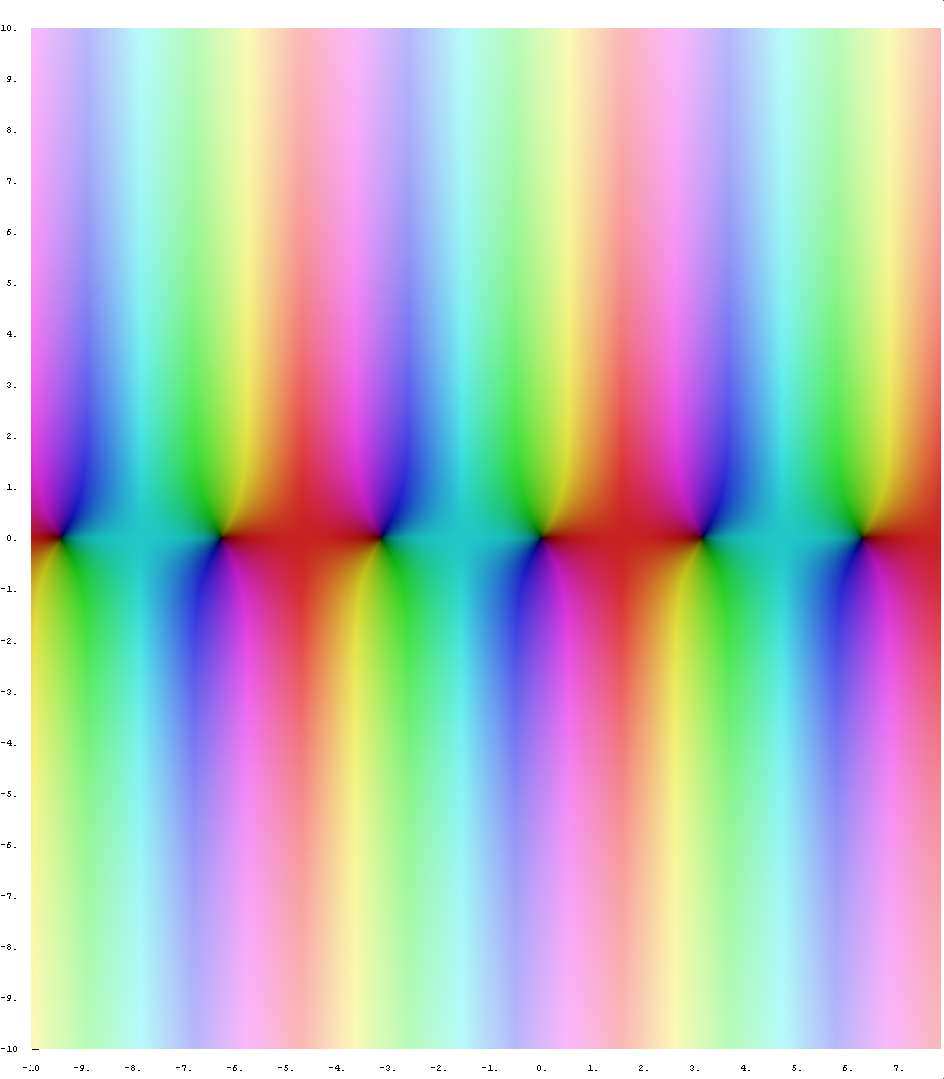
\includegraphics[scale=0.2]{sin_z}
		\caption{A domain colouring of $\sin (z)$ where brightness indicates $\left\lvert \sin (z) \right\rvert $ and hue indicates $\arg(\sin (z))$.}
	 \end{center}
\end{figure}
The differential equation
\begin{align*}
	a \frac{d^2y}{dz^2}+ b \frac{dy}{dz}+cy =0
\end{align*}
has a solution $y=e^{\lambda z} $. For instance, if
\begin{align*}
	\frac{d^2y}{dz}+2\frac{dy}{dz}+2y =0,
\end{align*}
then
\begin{align*}
	\lambda ^2 + 2\lambda + 2 =0,
\end{align*}
so $\lambda = -1\pm i$. Thus, the solutions to this differential equation are $y=e^{-(1+i)z}$ and $y = e^{-(1-i)z}$.\footnote{One may write these in terms of $\cos$ and $\sin$.}

Complex numbers simplify Fourier series. If $f(z) =f(2\pi+z)$, one can write
\begin{align*}
	f(z) &=  \sum_{n>0}^{} a_n\sin (nz) + \sum_{n>0}^{} b_n\cos (nz)\\
	     &= \sum_{n\in\Z}^{} c_ne^{inz},\ c_n\in \C.
\end{align*}

The function
\begin{align*}
	\tan (z): = \frac{\sin (z)}{\cos (z)}
\end{align*}
is defined in the natural way. On the upper half plane $\mathfrak H$, $\tan (z) \approx i$, and, on the lower half plane, $\tan (z) \approx -i$. Near the real axis, $\tan (z)$ oscillates as it does in the real case.\footnote{In real analysis, one thinks of $\sin$ and $\cos$ as being bounded and $\tan$ as being ``wild,'' and, in complex analysis, it is approximately the opposite.}

 \begin{exercise}\label{}\text{}
Express $\arccos (z)$ using $\log$ and $\sqrt{} $.
\end{exercise}

Notice that 
\begin{align*}
	\sin (iz) &= i\sinh (z);\\
	\cos (iz) &= \cosh (z);\\
	\tan (iz) &= i\tanh (z).
\end{align*}

\section{Holomorphic functions}
A function $f:\R\longrightarrow \R$ is called differentiable at $z_0\in \R$ if and only if $f$ is approximately linear there: That is, 
\[
	f(z)= f (z_0)+a (z-z_0) + \textrm{small error}
\]
.\footnote{``Small error'' means less than any nonzero linear function, or $\mathrm{error}/(z-z_0)$ goes to $0$ as $z$ goes to $z_0$.} Equivalently, $f$ is differentiable at $z_0$ if and only if some limit exists. 

Suppose that $w=u+iv$ is a function of $z=x+iy$.\footnote{Where $u$ and $v$ are functions of $x$ and $y$.} One writes $u$ and $v$ in a vector that one wants to be approximately linear:
 \begin{align*}
	 \mat{u(x,y) \\ v (x,y)} = \mat{u (x_0,y_0) \\ v (x_0,y_0)} + \mat{\partial u/\partial x&\partial u/\partial y\\ \partial v/\partial x&\partial v / \partial y}\mat{x-x_0\\y-y_0} + \mathrm{error}.
\end{align*}
One can approximate $w$ as a linear function. There's nothing really complex going on yet.

Now, one seeks a complex derivative. The function $w$ is differentiable if and only if
\begin{align*}
	w(z) = w (z_0) + \alpha(z-z_0) + \textrm{small error}.
\end{align*}
Here, $\alpha$ is a complex number. Hence, for $w$ to be differentiable as a complex function,\footnote{From the real two-variable case above.} one must also have
\begin{align*}
	\mat{\partial u/\partial x&\partial u/\partial y\\ \partial v/\partial x&\partial v / \partial y} = \mat {\Re (\alpha)&- \Im (\alpha)\\ \Im (\alpha) & \Re (\alpha)}.
\end{align*}
That is,
\begin{align*}
	\frac{\partial u}{\partial x} &= \frac{\partial v}{\partial y};\\
	\frac{\partial v}{\partial x}& = - \frac{\partial u}{\partial y}.
\end{align*}
These are the \defn{Cauchy--Riemann equations}\index{Cauchy--Riemann equations}. One also has the expected limit definition:
\begin{align*}
	\lim_{z\to z_0} \frac{w(z) - w (z_0)}{z-z_0}.
\end{align*}

\begin{definition}[ ]\label{}\text{}
Suppose that $w$ is a complex function of $z\in U\subset \C$ where $U$ is an open set of $\C$. The function $w$ is called \defn{holomorphic}\index{holomorphic function} if and only if it has a complex derivative everywhere.\footnote{That is, it is continuous with real derivatives satisfying the Cauchy--Riemann equations.}
\end{definition}

\begin{remark}
	Sometimes, one will see ``analytic'' instead of ``holomorphic.'' A function is \defn{analytic}\index{analytic function} if and only if it has a power series expansion at each point. Complex functions are holomorphic if and only if they are analytic. 
\end{remark}

There is another way of getting the Cauchy--Riemann equations. One defines
\begin{align*}
	\partial/\partial z &:= \frac{1}{2}(\partial/\partial x -  i\partial/\partial y);\\
		\partial/\partial \overline{z} &:= \frac{1}{2}(\partial/\partial x + i \partial/\partial y).
\end{align*}
These are \defn{Wirtinger derivatives}\index{Wirtinger derivatives}, which are chosen such that 
\begin{align*}
	(\partial /\partial z)z = 1;\  (\partial /\partial z) \overline{z} = 0;\  (\partial /\partial \overline{z}) z = 0;\  (\partial /\partial \overline{z})\overline{z} =1. 
\end{align*}
Hence, the Cauchy--Riemann equations are equivalent to
\begin{align*}
	\frac{\partial w}{\partial \overline{z}} = 0.
\end{align*}

\begin{remark}
Informally, ``holomorphic'' means ``depends on $z$ but not on $\overline{z}$.'' 
\end{remark}

\begin{example}[Holomorphic functions]\label{}\text{}
\begin{itemize}
	\item The functions  $1$ and $z$ are holomorphic.\footnote{They are linear.}
	\item Suppose that $f$ and $g$ are holomorphic on $U\subset \C$. Then, $f+g$, $f-g$, $fg$, $f/g$, and $f\circ g$ are holomorphic.
	\item If a power series $a_0 + a_1z + a_2z^2 + \cdots$ converges for $\left\lvert z \right\rvert <r$, then it is holomorphic and its derivative is $a_1 + 2a_2z + \cdots$.
	\item Hence, $\sin$, $\cos$, $\tan$, $\exp$, and $\log$ are holomorphic when defined.
	\item If $f$ is holomorphic, then its derivative is.
\end{itemize}
\end{example}

\begin{example}[Non-holomorphic functions]\label{}\text{}
\begin{itemize}
	\item $\Re (z)$;
	\item $\Im (z)$;
	\item $\left\lvert z \right\rvert$;
	\item $\left\lvert z \right\rvert ^2$;
	\item $\overline{z}$.
\end{itemize}
\end{example}

What polynomials in $x$ and $y$ are holomorphic? Equivalently, what polynomials in $z=x+iy$ and $\overline{z}=x-iy$ are holomorphic? When is $\sum_{}^{} a_{mn}z^m \overline{z}^n$ holomorphic? 
One needs
\begin{align*}
	\partial/\partial \overline{z}= \sum_{}^{} a_{mn} z^m n \overline{z}^{n-1} = 0,
\end{align*}
so $a_{mn} n = 0$ for all $m$ and $n$, hence $a_{mn} = 0$ if $n>0$. Therefore, $f(x,y)=  \sum_{}^{} a_{m0}z^m$ is a polynomial in $z$.

\section{Harmonic functions}
Suppose that $w=u+iv$ is a complex function of $ z=x+iy$. Given a function $u$ of $x$ and $y$, can one find a holomorphic function $w$ such that $u = \Re(w)$? In general, no. If a complex function is holomorphic, it satisfies the Cauchy--Riemann equations:
\begin{align*}
	\frac{\partial u}{\partial x} &= \frac{\partial v}{\partial y};\\\frac{\partial v}{\partial x}& = - \frac{\partial u}{\partial y}.
\end{align*}
These imply that
\begin{align*}
	\frac{\partial^2 u}{\partial x^2} = \frac{\partial^2y}{\partial x \partial y} = -\frac{\partial^2 u}{\partial y^2}.
\end{align*}
In particular,
\begin{align*}
\frac{\partial ^2 u}{\partial x^2} + \frac{\partial^2 u}{\partial y^2} = 0.
\end{align*}
This is the \defn{Laplace equation}\index{Laplace equation}, and functions that satisfy it are called \defn{harmonic functions}\index{harmonic function}. It has a physical interpretation: It gives the steady state heat of some planar region.\footnote{Equivalently, one writes $\nabla u=0$.} 

We use this to find solutions to the Laplace equation by taking a holomorphic function and taking its real or imaginary part.
\begin{example}[Find all harmonic polynomials in $x$ and $y$]\label{}\text{}
The polynomials that result from taking the real and imaginary parts of powers of $z = x+iy$ are harmonic, and they happen to be a basis for harmonic polynomials.
\end{example}

\begin{example}[ ]\label{}\text{}
The function
\begin{align*}
	ze^z = (x+iy)e^x (\cos y + i\sin y)
\end{align*}
is holomorphic. Therefore, its real part, $e^x(x\cos y - y\sin y)$, is harmonic.
\end{example}

Is any harmonic function $u$ the real part of some holomorphic function $w = u+iv$? It is useful to take $u$ as a function on an open set $U\subset \C$. The answer depends on $U$. 

One is trying to solve the Cauchy--Riemann equations. These determine $v$ up to a constant. 

\begin{problem}
	Given functions $f$ and $g$ of $x$ and $y$, can one solve $\partial v/\partial x = f$ and $\partial v/\partial y = g$?
\end{problem}

One needs
\[
	\frac{\partial f}{\partial y} = \frac{\partial f}{\partial x}
\] 
because both sides equal $\partial^2 v/\partial x\partial y$. Sometimes, one can solve for $v$. 
Suppose that $U$ is a rectangle containing the origin. Put $v(0,0)=0$. One sees that
\begin{align*}
	v(x,0) =  \int_{0}^{x} f(x,0)   \, dx 
\end{align*}
and
\begin{align*}
	v(x,y) &= v (x,0) +  \int_{0}^{y} g(x,y)  \, dy. 
\end{align*}
Clearly, $\partial v/\partial y=g$. Is $\partial v/\partial x = f$? This is true on the $x$ axis by definition. Further, one gets
\begin{align*}
	\frac{\partial v}{\partial x} &= \frac{\partial}{\partial x} v(x,0) +  \int_{0}^{y} \frac{\partial g}{\partial x}(x,y)  \, dy\\
				      &= f(x,0) +  \int_{0}^{y} \frac{\partial f}{\partial y}  \, dy\\
				      &= f(x,y),
\end{align*}
so $\partial v/\partial x = f$.

Suppose that one is given a harmonic function $u$ on a rectangle. Then, one can find $w=u+iv$ where $w$ is holomorphic. One needs to solve $\partial v/\partial y =\partial u /\partial x = g$ and $\partial v/\partial y = -\partial u/\partial y = f$. One needs $\partial g/\partial x = \partial f/\partial y$, and this follows from $u$ being harmonic.

What about other regions? Suppose that $U = \C-\{0\}$. Take $u=\log (r)$. The function $u$ is harmonic\footnote{It is, more or less, the fundamental solution of the Laplace equation.} except at $x=y=0$. Further, $u = \Re (\log (z))$, and one takes $v = \Im(\log (z)) = \arg (z)$. However, $\log (z)$ is not defined on all of $U$ since $\arg (z)$ is not defined.\footnote{If one takes a disk and ``extends'' it into a bigger region by taking disks that overlap in a circular formation around some point, one gets a problem when the last disk overlaps the original one: Is $\arg (z)$ near $0$ or $2\pi$? This is the problem of being defined up to a constant.} If a region $U$ has ``holes,'' then one cannot extend a harmonic function $u$ to a holomorphic function $w$. 

If $U$ is simply connected, then any harmonic function $u$ is the real part of a holomorphic function $w$ where $\Im(w)$ is unique up to a constant.

In differential geometry, one might write
\begin{align*}
	\partial v /\partial x = f,\ \partial v / \partial y = g
\end{align*}
as a $1$-form 
\begin{align*}
	dv = (\partial v/\partial x)dx +  (\partial v/\partial y) dy.
\end{align*}
Does there exist a $v$ such that $ dv =\omega = f\,dx + g\,dy$? We need $d\omega = 0$, or $df/dy = dg/dx$. We saw that $\omega = dv$ for some $v$ if and only if $dv = 0$ on a simply connected region $U$.

\begin{definition}[ ]\label{}\text{}
The \defn{de Rham cohomology group}\index{de Rham cohomology group} of an open region $U$  of the complex numbers, $H^1(U)$, is the set of closed $1$-forms $\omega$\footnote{$d\omega = 0$.} modulo the set of exact forms $\omega$.\footnote{$\omega = dv$ for some $v$.}
\end{definition}

We have shown that, if $U$ is simply connected, then $H^1(U)=0$. 
\section{Integration}
We cannot really integrate a complex function $f$ from $\alpha$ to $\beta$ since there are many paths between them. So, we define an integral over a path $C$ from $\alpha$ to $\beta$.

If $\alpha$ and $\beta$ are real and we consider the path along the real line, we write $f = g + ih$ for real functions $g$ and $h$, and then we have
\begin{align*}
	\int_{\alpha}^{\beta} f(z)  \, dz = \int_{\alpha}^{\beta} g(x)  \, dx + i \int_{\alpha}^{\beta} h(x)  \, dx.   
\end{align*}

Recall that an integral is a ``sum.''

A path $C$ from $\alpha$ to $\beta$ is given by a function $\rho :[r,s] \longrightarrow \C$ where $\rho(r)=\alpha$ and $\rho(s)= \beta$. Now suppose that $\rho$ has a continuous derivative and we consider 
\begin{align*}
	\int_{C}^{} f(z)  \, dz. 
\end{align*}
We write $z=\rho(x)$ and $dz = \rho'(x) \,dx$ (the proof of this is similar to that in the real case). Hence
\begin{align*}
	\int_{C}^{} f(z)  \, dz= \int_{r}^{s} f(\rho(x)) \rho'(x) \, dx  
\end{align*}
This is an alternative definition (to the ``limit of a sum'' one).

Now write $f=u+iv$ and $z=x+iy$. We can write a complex integral as a path integral:
 \begin{align*}
	 \int_{C}^{} f(z)  \, dz &= \int_{C}^{} (u+iv) \,(dx+idy) \\
				 &= \int_{C}^{} u  \, dx - v\,dy + i \int_{C}^{} v\,dx + u  \, dy.  
\end{align*}

Notice that
\begin{align*}
	\int_{C}^{} f(z)  \, dz 
\end{align*}
is almost independent of the parameterization $\rho$ since the summands of the integral are independent of the parameterization. However, we need to pay attention to the direction of the path (that is, if $\rho (r) = \beta$ and $\rho(s) = \alpha$). In this case, a sign changes.

Some properties:
\begin{itemize}
	\item \begin{align*}
		\int_{C_1}^{} f(z)  \, dz + \int_{C_2}^{} f(z)   \, dz = \int_{C_1\cup C_2}^{} f(z)  \, dz;   
	\end{align*}
\item \begin{align*}
	\int_{C}^{} f(z) +g(z) \, dz = \int_{C}^{} f(z)  \, dz + \int_{C}^{} g(z)  \, dz  ; 
\end{align*}
\item If $M$ is an upper bound for $\left\lvert f \right\rvert $ and $\left\lvert C \right\rvert $ is the length of $C$, then
	\begin{align*}
		\left\lvert \int_{C}^{} f(z)  \, dz  \right\rvert \le M\left\lvert C \right\rvert.
	\end{align*}
\end{itemize}

\begin{example}[ ]\label{}\text{}
Compute
	\begin{align*}
	\int_{C}^{} z^n  \, dz 
\end{align*}
where $C$ is a path from $1$ to $1$. If $C$ is the trivial path (the parameterization $\rho=1$), then (clearly) 
\begin{align*}
	\int_{C}^{} z^n  \, dz = 0. 
\end{align*}
Instead, if $C$ is given by 
\begin{align*}
	\rho : [0,2\pi] \longrightarrow \C : \alpha \longmapsto e^{i\alpha},
\end{align*}
then
\begin{align*}
	\int_{C}^{} z^n  \, dz &= \int_{0}^{2\pi} e^{inx} i e^{ix}  \, dx\\
			       &= i \int_{0}^{2\pi} e^{i(n+1)x}  \, dx\\
			       &=
			       \begin{cases}
				       2\pi i & n=-1\\
				       0 &\textrm{otherwise}.
			       \end{cases}
\end{align*}
So the integral does depend on the path.
\end{example}

\section{Cauchy's theorem}
\begin{theorem}[Cauchy]\label{}\index{Cauchy's theorem}\text{}
Suppose $C_1$ and $C_2$ are homotopic paths and $w$ is holomorphic. Then
\begin{align*}
	\int_{C_1}^{} w(z)  \, dz = \int_{C_2}^{} w(z)  \, dz.  
\end{align*}
\end{theorem}

Recall that ``homotopic'' means you can slide one path into the other while keeping the endpoints fixed. 
\begin{theorem}[Cauchy]\label{}\index{Cauchy's theorem}\text{}
Suppose $C$ is homotopic to a constant curve and $w$ is holomorphic (in $C$). Then
\begin{align*}
	\int_{C}^{} w(z)  \, dz = 0. 
\end{align*}
\end{theorem}

One can see that these are equivalent. We will prove a weaker version, and we will use Green's theorem. 
\begin{theorem}[Green]\label{}\index{}\text{}
\begin{align*}
	\oint_C f(x,y)\,dx +  g (x,y) \, dy = \iint_D \frac{\partial g}{\partial x} - \frac{\partial f}{\partial y} \, dx\, dy
\end{align*}
where $D$ is the interior of $C$.
\end{theorem}

Hence 
\begin{align*}
	\int_{C}^{} w(z)  \, dz &=\int_{C}^{} (u+iv) (dx+i\,dy) \\
				&= \int_{C}^{} u\,dx - v  \, dy + i \int_{C}^{} u\, dy + v  \, dx\\
				&= \iint_D \frac{\partial u}{\partial y} - \frac{\partial v}{\partial x}\,dx\,dy + i \iint_D \frac{\partial v}{\partial y} - \frac{\partial u}{\partial x}\,dx\,dy\\
				&= 0.
\end{align*}

\begin{enumerate}
	\item In a simply connected region, a holomorphic function $w$ has an antiderivative. One might define it as
		\begin{align*}
			\int_{\alpha}^{z} w(z)  \, dz, 
		\end{align*}
		but is this well defined? There are many paths from $\alpha$ to $z$. Since the region is simply connected, any two paths from $\alpha$ to $z$ are homotopic, so the integrals are the same. 
	\item What is 
		\begin{align*}
			\int_{C}^{} \frac{z^2+3}{z^4-2z+3}  \, dz 
		\end{align*}
		where $C$ is the circle of radius $2$? One cannot apply just Cauchy's theorem, since $z^4-2z+3$ has roots inside $C$. (In particular it is not holomorphic.) Instead, let $C$ be the circle of radius $R>2$. One sees that
		\begin{align*}
			\int_{C}^{} \frac{z^2 + 3}{z^4-2z+3}  \, dz &\le 2\pi R \cdot (2/R^2) \\
								    &\le 4\pi/R
		\end{align*}
		for all real $R>2$. Hence the integral is $0$.
\end{enumerate}
\section{Cauchy's integral formula}
If $f$ is holomorphic in $U$, then 
\begin{align*}
	f(w)=  \frac{1}{2\pi i} \int_{C}^{} \frac{f(z)}{z-w}  \, dz 
\end{align*}
where $C$ goes around $w$ once counterclockwise. 
\begin{proof}
Write
\begin{align*}
	f(z) = \textrm{constant} + g (z)
\end{align*}
where $g(0)=0$. If $f$ is constant we need to show that
\begin{align*}
	\int_{C}^{} 1/z  \, dz = 2\pi i 
\end{align*}
If we let $C$ be a circle of radius $r$ and $z=re^{i\theta}$ then
\begin{align*}
	\int_{C}^{} 1/z  \, dz &= \int_{0}^{2\pi} r^{-1}e^{-i\theta} r ie^{i\theta}  \, d\theta\\
			       &= 2\pi i.
\end{align*}
If $g$ vanishes at $0$, we want to show that 
\begin{align*}
	\int_{C}^{} \frac{g(z)}{z}  \, dz = 0. 
\end{align*}
Now we let $C$ be a circle of small radius $r$. Then if $\varepsilon$ is an upper bound for $g$
\begin{align*}
	\int_{C}^{} \frac{g(z)}{z}  \, dz & \le \left\lvert C \right\rvert \sup \left\lvert g(z)/z \right\rvert \\
					  &\le 2\pi r (\varepsilon/r) \\
					  &=2\pi \varepsilon.
\end{align*}
\end{proof}

\begin{enumerate}
	\item Given a holomorphic function on a contour $C$, $f$ is determined inside $C$.
	\item Suppose $f$ is defined on a disk $U$. Then 
		\begin{align*}
			\left\lvert f(w) \right\rvert \le\sup_{z\in \partial U} f(z).
		\end{align*}
	\item We know that
		\begin{align*}
			f(w) =  \frac{1}{2\pi i} \int_{C}^{} \frac{f(z)}{z-w}  \, dz. 
		\end{align*}
		Then taking the $n$th derivative 
		\begin{align*}
			f^{ (n)}  (w) =  \frac{1}{2\pi i} \int_{C}^{} \frac{f(z)}{(z-w)^{n+1}} n! \, dz. 
		\end{align*}
		Differentiating under the integral sign is valid because $C$ has finite length and $f(z)/ (z-w)$ has continuous derivatives near $C$. So the $n$th derivative of $f$ exists! That is, if $f$ is differentiable (in an open region) then it is infinitely differentiable.
\end{enumerate}
\begin{theorem}[Liouville]\label{lvl}\index{}\text{}
If $f$ is bounded and holomorphic in $\C$ then $f$ is constant.
\end{theorem}
\begin{proof}
Suppose $C$ is a circle of large radius $R$. We know that
\begin{align*}
	f'(w) =  \frac{1}{2\pi i}\int_{C}^{} \frac{f(z)}{(z-w)^2}  \, dz. 
\end{align*}
Then 
\begin{align*}
	\left\lvert f'(w) \right\rvert &\le (1/2\pi)  (2\pi R)  (\sup f)/R^2 \\
				       &\le \frac{\sup f}{R}.
\end{align*}
Since $f$ is bounded, $f'(w)=0$ at all $w$. Hence $f$ is constant.
\end{proof}

\begin{exercise}\label{}\text{}
Suppose $\left\lvert f \right\rvert$ is bounded by some $g\in \C[z]$. Show that $f$ is a polynomial.
\end{exercise}
\begin{enumerate}
	\setcounter{enumi}{3}
	\item Any holomorphic function can be expanded as a power series. (This is not true for the real function
		\begin{align*}
			f(z) = 
			 \begin{cases}
				 0  & x=0\\
				 e^{-1/z^2} &\textrm{otherwise}
			\end{cases}
		\end{align*}
		though it is infinitely differentiable.)
\end{enumerate}

Suppose the Taylor series $\sum_{k}^{} a_kz^k$ converges for some $z_0$. Then $a_nz_0^n$ is bounded, and $\sum_{k}^{} a_kz^k$ converges if $\left\lvert z \right\rvert <\left\lvert z_0 \right\rvert $. (The series converges if $\left\lvert z \right\rvert < R$ and diverges if $\left\lvert z \right\rvert > R$. Don't ask about what happens when $\left\lvert z \right\rvert =R$.)

\begin{theorem}[Morera]\label{}\index{}\text{}
If 
\begin{align*}
	\int_{C}^{} f(z)  \, dz = 0 
\end{align*}
then $f$ is holomorphic.
\end{theorem}
\begin{proof}
Define
\begin{align*}
	F(z) :=  \int_{a}^{z} f(z)  \, dz. 
\end{align*}
This is well-defined. Then check that $F$ has a derivative $f$. So $F$ is holomorphic, and $F'=f$ is holomorphic.
\end{proof}


\section{Analytic continuation}
Suppose $U$ is a connected open set and $f$ is holomorphic on $U$. If you know what $f$ is on any subregion of $U$, then $f$ is determined uniquely on the rest of $U$. (What?!)

The point is that if $f$ is holomorphic on $U$ and $f$ is not identically $0$ then the roots of $f$ are discrete in $U$ (no limit points in $U$).

Suppose $0$ is a limit point of the roots of $f$ with $0\in U$. Then  $f=0$ near $0$. Otherwise, 
\begin{align*}
	f(z) =  a_nz^n + a_{n+1}z^{n+1} + \cdots,
\end{align*}
and we can assume that $a_n \ne 0$. So 
\begin{align*}
	f(z) = z^n (a_n + a_{n+1}z + \cdots),
\end{align*}
and the parenthetical sum is continuous and nonzero at $z=0$, so it is nonzero near $z=0$. This contradicts that $0$ is a limit point of the roots of $f$. 

Now let $V$ be the largest open subset of $U$ with $f=0$ on $V$. Then $V$ is closed under taking limits by the above. And $V$ is nonempty because we assumed that there was some limit point of roots of $f$, so $V$ is closed and open. Therefore $V=\emptyset$ or $V=U$ since $U$ is connected, but $V$ is nonempty, so $V=U$. So $f$ is identically $0$. 

Now suppose $f=g$ on some set $S$ with a limit point in $U$. Then $f-g=0$ on $S$, so $f-g=0$ (otherwise we get a nonzero holomorphic function with roots having a limit point in $U$). So $f=g$. \hfill \qed

This is true for real analytic functions. 

Suppose $f$ is holomorphic on an open nonempty set $V$ and $U\supseteq V$ is connected. Then there is at most one way to extend $f$ to $U$. This ``extension'' is called the function's  \defn{analytic continuation}\index{analytic continuation}.

\begin{example}[Gamma function]\label{}\text{}
Recall 
\begin{align*}
	\Gamma(s) :=  \int_{0}^{\infty} e^{-t}t^{s-1}  \, dt. 
\end{align*}
This is holomorphic for $\Re s > 0$. We can differentiate under the integral sign since $e^{-t}t^{s-1}$ has continuous derivative and is rapidly decreasing. Since 
\begin{align*}
	\Gamma (s) =  \frac{\Gamma(s+1)}{s},
\end{align*}
we can analytically continue $\Gamma$ for $\Re s>-1$ ($s\ne 0$) and repeat this process such that $\Gamma(s)$ is holomorphic for all nonpositive integers $s$.
\end{example}

\begin{example}[ ]\label{}\text{}
Consider the function $\log z$ for $\Re z > 0$. You can continue $\log$ such that $\log(-1) = \pm \pi i$ depending on the region you choose. 
\end{example}

\begin{example}[Riemann zeta function]\label{}\text{}
Recall 
\begin{align*}
	\zeta(s) :=  \sum_{k}^{} 1/k^s.
\end{align*}
But $\zeta$ converges for $\Re s > 1$. We will show that $\zeta$ is holomorphic next section, so for now we will take that for granted. But $\zeta(s)-  ({2}/{2^s})\zeta(s)$ converges for $\Re s > 0$ to a holomorphic function (which we will show next time), so we can continue $\zeta$ as follows:
 \begin{align*}
	\frac{1}{1-2/2^s}\left(\zeta(s)- \frac{2}{2^s}\zeta(s)\right)
\end{align*}
\end{example}

\section{Locally uniform convergence}
Suppose $f_1,f_2,\hdots$ are holomorphic on $U$. Does $\sum_{i}^{} f_i$ converge and is it holomorphic? We want to know whether the sequence of partial sums $(g_n)$ of this series converges.

There are some useful notions of convergence.
\begin{enumerate}
	\item We say $g_n(z)\to g (z)$ \defn{pointwise}\index{pointwise convergence} if
		\begin{align*}
			\lim_{n\to\infty} g_n(z) = g (z)
		\end{align*}
		for all $z$. This is too weak.
	\item We say $g_n\to g$ uniformly if $g_n$ tends to $g$ roughly at the same rate at all points. This is too strong.
	\item We can have $g_n\to g$ uniformly on compact sets, and this is just right.
\end{enumerate}

Consider pointwise convergence. We would like
\begin{align*}
	\int_{}^{} \lim g_n = \lim \int_{}^{} g_n. 
\end{align*}
We can construct a Dirac delta--like sequence of functions such that $\lim_{n\to\infty}g_n(z) =0$ for all $z$ and the integral is $1$. And the limit of continuous functions need not be continuous. This makes pointwise convergence problematic.

Uniform convergence is more like having 
\begin{align*}
	\lim_{n\to\infty} \sup_z (g_n(z)-g (z)) =0
\end{align*}
for all $z$.
\begin{definition}[Uniform convergence]\label{}\text{}
A sequence of functions $(g_n)$ \defn{converges uniformly}\index{uniform convergence} to a function $g$ if for all $\varepsilon > 0$ there exists a natural number $N$ such that for all $z$ and $n\ge N$
\begin{align*}
 \left\lvert g_n(z) - g (z) \right\rvert <\varepsilon.
\end{align*}
\end{definition}

A sequence of functions converges pointwise to $g$ if for all $\varepsilon >0$ and all $z$ there exists a natural number $N$ such that for all $n\ge N$ we have $\left\lvert g_n(z) -g(z)\right\rvert <\varepsilon$.

\begin{remark}
	If $g_n\to g$ uniformly then 
	\begin{align*}
		\int_{a}^{b} g_n(z)  \, dz \longrightarrow \int_{a}^{b} g(z)  \, dz.  
	\end{align*}
	(This is a finite interval.)
\end{remark}
\begin{remark}
	If $g_n\to g$ uniformly and $g_n$ is holomorphic then $g$ is holomorphic.
\end{remark}
\begin{proof}
Suppose $g_n$ is holomorphic. Then 
\begin{align*}
	\int_{C}^{} g_n(z)  \, d z = 0
\end{align*}
by Cauchy's theorem. This implies that 
\begin{align*}
	\int_{C}^{} g(z)  \, dz =0
\end{align*}
by uniform convergence. Hence $g$ is holomorphic by Morera's theorem.
\end{proof}

\begin{warn}
	In real analysis, the uniform limit of analytic functions does not need to be analytic.
\end{warn}

\begin{problem}
	The series
	\begin{align*}
		\sum_{k}^{} z^k = \frac{1}{1-z}
	\end{align*}
	is not uniform on $\left\lvert z \right\rvert <1$. The error 
	\begin{align*}
		\left\lvert z^n + z^{n+1} + z^{n+1} + \cdots \right\rvert = \frac{z^n}{1-z}
	\end{align*}
	is rather large for $z\approx 1$. We want an upper bound for the error that does not depend on $z$. Take $\left\lvert z \right\rvert <1/2$. Then 
	\begin{align*}
		\left\lvert \frac{z^n}{1-z} \right\rvert \le (1/2)^{n-1}
	\end{align*}
	tends to $0$ independent of $z$. We can do this for $0.9$, $0.99$, etc. We want $\lim g_n$ to be holomorphic (locally). So we just need $g_n\to g$ uniformly on some neighbourhood of each point. We call this \defn{local uniform convergence}\index{local uniform convergence}. The example above is locally uniform convergent. Again, it is uniform convergence on compact subsets of $U$. (That local uniform convergence is equivalent to uniform convergence on compact subsets comes from $\C$ being locally compact.) 
\end{problem}

Suppose the power series $a_0 + a_1z + a_2z^2 + \cdots$ converges for $\left\lvert z \right\rvert <R$. We want to show that it is holomorphic for $\left\lvert z \right\rvert < R$. Suppose $r<s<R$. We will show that convergence is uniform for $\left\lvert z \right\rvert < r$. We know that $a_ns^n$ is bounded, so $a_n \le M/s^n$ for some fixed $M$. So $\left\lvert a_nr^n \right\rvert \le M(r/s) ^n$. And $r/s<1$, so
\begin{align*}
	\left\lvert a_nz^n + a_{n+1}z^{n+1} + \cdots \right\rvert &\le M((r/s) ^n +(r/s)^{n+1} + \cdots ) \\
								  &\le M\frac{(r/s)^n}{1-r/s}
\end{align*}
 independent of $z$. This tends to $0$, and this gives uniform convergence since we found a bound tending to $0$ independent of $z$. So the limit is holomorphic.

One can check that the Riemann $\zeta$ function converges for $\Re s>1$. But this convergence is not uniform. It is uniform in the region $\Re s>s_0$ for some fixed $s_0>1$. This is because the error is given by
\begin{align*}
	\frac{1}{\left\lvert m \right\rvert ^s} + \frac{1}{\left\lvert m+1 \right\rvert ^s} + \cdots \le \frac{1}{m^{s_0}} + \frac{1}{(m+1)^{s_0}} + \cdots,
\end{align*}
which tends to $0$. We see that $\zeta$ is holomorphic for $\Re s>1$ since the union of the regions on which it converges is $\Re s > 1$.

The series
\begin{align*}
	\frac{1}{1^s} - \frac{1}{2^s} + \frac{1}{3^s} -\frac{1}{4^s}+\cdots
\end{align*}
certainly converges for real $s>0$, but what about in general?

\begin{proposition}[ ]\label{}\text{}
Suppose \begin{align*}
	\frac{a_1}{1^s} + \frac{a_2}{2^s} + \cdots
\end{align*}
converges for $s=s_0$. Then it converges uniformly in a region that can be made arbitrarily close to $\Re s>0$ such that it is holomorphic in the region $\Re s>\Re s_0$.
\end{proposition}
\begin{remark}
	[Abel's theorem] We can write
	\begin{align*}
	&\phantom{=}\ \	a_mb_m+ a_{m+1} b_{m+1} + \cdots+a_nb_n\\ &= (b_m - b_{m+1}) a_m +  (b_{m+1} - b_{m+2}) (a_m + a_{m+1}) + \cdots +  (b_n - 0) (a_m + a_{m+1} + \cdots + a_n).
	\end{align*}
\end{remark}
\begin{remark}
	\begin{align*}
		\left\lvert \frac{1}{(m+1) ^s} - \frac{1}{m^s} \right\rvert \le \left(\left\lvert \frac{1}{m^s}  \right\rvert - \left\lvert \frac{1}{(m+1)^s} \right\rvert \right) \frac{\left\lvert s \right\rvert }{\Re s}
	\end{align*}
\end{remark}
\begin{proof}
Let's take $s_0=0$. We know that $a_1+a_2+a_3+\cdots$ converges, and we want to show that \begin{align*}
	\frac{a_1}{1^s} + \frac{a_2}{2^s} + \cdots
\end{align*}
converges uniformly in the region that can be made arbitrarily close to the region $\Re s > 0$. If $m$ is sufficiently large then the partial sums $a_m +\cdots +a_n$ will be less than some $\varepsilon > 0$. We get 
\begin{align*}
	&\phantom{=}\ \ \left\lvert \frac{a_m}{m^s} + \frac{a_{m+1}}{(m+1)^s} + \cdots + \frac{a_n}{n^s} \right\rvert \\
	&= a_m \left( \frac{1}{m^s} - \frac{1}{(m+1)^s} \right) + (a_m + a_{m+1}) \left( \frac{1}{(m+1)^s} -  \frac{1}{(m+2)^s} \right) + \cdots + (a_m + \cdots + a_n)  \frac{1}{n^s}\\
	&\le \varepsilon \frac{\left\lvert s \right\rvert }{\Re s} \left\lvert \frac{1}{m^s} \right\rvert, 
\end{align*}
and this is bounded for some $s$ in the region approximating $\Re s> 0 $, so that Dirichlet series converges uniformly on that region. Hence these Dirichlet series are holomorphic for $\Re s > 0$.
\end{proof}

\section{Residue calculus}
\begin{theorem}[ ]\label{}\index{}\text{}
Suppose $f$ is holomorphic except at finitely many points $a_k$. Then 
\begin{align*}
	\int_{C}^{} f(z)  \, dz = 2\pi i \sum_{k}^{} \Res(f, a_k)  
\end{align*}
where the residue at $a_k$
\begin{align*}
	\Res(f, a_k) := \frac{1}{2\pi i} \int_{C_k}^{} f(z)  \, dz 
\end{align*}
and $C_k$ is a small region around $a_k$.
\end{theorem}

This makes sense. But what is the residue of $f(z)\,dz$ at a point $p$? We expand $f$ as a Laurent series:
\begin{align*}
	f(z) = a_{-n}(z-p)^{-n} + \cdots + a_{-1}(z-p)^{-1} + a_0 +  a_1(z-p) + \cdots.
\end{align*}
Then 
\begin{align*}
	\Res(f, p) = a_{-1}.
\end{align*}
Take $p=0$. Recall that
\begin{align*}
	\int_{C}^{} z^n  \, dz = 
	\begin{cases}
		2\pi i &n=-1\\
		0&\textrm{otherwise.}
	\end{cases}
\end{align*}

\begin{enumerate}
	\item We can transform a contour integral into a sum of residues;
	\item We can transform a sum into a contour integral.
\end{enumerate}

\begin{example}[ ]\label{}\text{}
\begin{align*}
	\int_{-\infty}^{\infty} \frac{1}{1+z^2}  \, dz. 
\end{align*}
Introductory methods show that this integral is $\pi$. A good contour to use is a semicircle from $-R$ to $R$ as $R\to \infty$. In the limit we can ignore the ``curved section'' of the semicircle. This is not holomorphic at $z = \pm i$, and $z=-i$ is not in the contour. Hence
\begin{align*}
	\int_{-\infty}^{\infty} \frac{1}{1+z^2}  \, dz &= 2\pi i \Res(f, i)\\
						       &= 2\pi i  (1/2i)\\
						       &= \pi.
\end{align*}
\end{example}

\begin{example}[ ]\label{}\text{}
\begin{align*}
	\int_{-\infty}^{\infty} \frac{\cos z}{1+z^2}  \, dz.
\end{align*}
The function $(\cos z)/ (1+z^2)$ does not have an elementary antiderivative. We \emph{cannot} use the semicircle since $(\cos z)/ (1+z^2)$ is large in the ``curved section'' (so we cannot ignore it). We can see that 
 \begin{align*}
	\int_{-\infty}^{\infty} \frac{\cos z}{1+z^2}  \, dz = \Re \int_{-\infty}^{\infty} \frac{e^{iz}}{1+z^2}  \, dz. 
\end{align*}
Since $\left\lvert e^{iz} \right\rvert \le 1$, the integral over the ``curved section'' approaches $0$ in the limit, so we ignore it. Hence this integral is $2\pi i\Res(f, i)$. We get
\begin{align*}
	\int_{-\infty}^{\infty} \frac{\cos z}{1+z^2}  \, dz &= 2\pi i \Res(f,i)\\
							    &= 2\pi i  (e^{-1}/2i)\\
							    &=\pi/e.
\end{align*}
\end{example}

\begin{example}[ ]\label{}\text{}
\begin{align*}
	\int_{-\infty}^{\infty} \frac{\sin z}{z}  \, dz. 
\end{align*}
The semicircle doesn't work again, since $\sin z$ is ``big'' on the curved section. Then we try
\begin{align*}
	\Im \int_{-\infty}^{\infty} \frac{e^{iz}}{z}  \, dz =  \int_{-\infty}^{\infty} \frac{\sin z}{z}  \, dz. 
\end{align*}
But at $z=0$, $(\cos z) /z$ is infinite. Also, $e^{iz}/z$ is holomorphic except at $z=0$. Now consider the semicircle contour, but we avoid the point $z=0$ with a smaller semicircle. The imaginary part of the integral on the ``straight section'' of this contour approaches
\begin{align*}
 \int_{-\infty}^{\infty} \frac{\sin z}{z}  \, dz. 
\end{align*}
We want to show that the ``outside curved section'' approaches $0$. In the ``middle part'' of this section $\left\lvert e^{iz} \right\rvert $ is small and on the ``ends'' $\left\lvert 1/x \right\rvert $ is small. Pick $M\in \R$ such that $\left\lvert e^{iz} \right\rvert <\varepsilon$ when $\Im z > M$. Then
\begin{align*}
	\int_{\textrm{above $M$}}^{} f(z)  \, dz &\le \varepsilon \pi\to 0
\end{align*}
and 
\begin{align*}
	\int_{\textrm{below $M$}}^{} f(z)  \, dz \le 2M(1/R) \to 0. 
\end{align*}
So we can ignore this section. Now consider the ``inside curved section,'' which is a semicircle of radius $r$. If $C$ is a circle around the origin, then
\begin{align*}
	\int_{C}^{} \frac{e^{iz}}{z}  \, dz = 2\pi i \Res(f,0) = 2\pi i. 
\end{align*}
If $D$ is the contour formed by the contour in question, then
\begin{align*}
	\int_{D}^{} \frac{e^{iz}}{z}  \, dz \to -\frac{1}{2} (2\pi i \Res(f,0)) = -\pi i.
\end{align*}
Hence 
\begin{align*}
\int_{-\infty}^{\infty} \frac{\sin z}{z}  \, dz = \pi. 	
\end{align*}
\end{example}

\section{Summing series}
\begin{example}[Basel problem]\label{}\text{}
Show that
\begin{align*}
	\sum_k 1/k^2 = \pi^2/6.
\end{align*}
We want to find a function whose residues correspond to $1/k^2$. The function $f(z) = 1/ (\tan z)$ has singularities at $\pi \Z$. The residues at each of these points is $1$ because for $z\approx 0$ then $\tan z \approx z$, so $1/(\tan z)\approx 1/z$, which has residue $1$. Now for $g(z) = 1/z^2 (\tan z)$, the residues at $\pi k$ is $1/(\pi k)^2$ for $k \in \Z- \{0\}$. Now at $0$, the pole is of order $3$. We see that
\begin{align*}
	\sum_k \Res(g,a_k) = \Res(g,0) + \frac{2}{\pi^2} \left( \sum_k 1/k^2 \right).
\end{align*}
Let's calculate the sum of the residues first (we want to show that this sum is $0$). Consider the contour $C$ given by a square with side length $2R$ centred at the origin where $R = \pi/2 + \pi k$. In particular, 
 \begin{align*}
	 \abs{\int_C \frac{1}{z^2\tan z} \, dz} &\le \abs{C} \max_C f\\
						&= 8R\left (\max_C {1}/{z^2}\right) \left(\max_C {1}/{\tan z}\right)\\
						&= 8R(1/R^2)M \to 0
\end{align*}
where $M$ is independent of $R$. Hence
\begin{align*}
	\sum_{k} \Res(g,a_k) \to 0.
\end{align*}
What about that mysterious residue? We see that
\begin{align*}
	\frac{1}{\tan z} &= \frac{\cos z}{\sin z}\\ &= \frac{ 1 - z^2/2! + \cdots}{z - z^3/3! + \cdots}\\
			 &\approx z\inv - z/3.
\end{align*}
So 
\begin{align*}
	\frac{1}{z^2\tan z} \approx z^{-3} - z\inv / 3.
\end{align*}
But recall that the residue is given by the coefficient of $z\inv$ in the Laurent series expansion. So $\Res (g,0) = -1/3$. Hence
\begin{align*}
	0 = -1/3 + \frac{2}{\pi^2} \left(\sum_k 1/k^2\right),
\end{align*}
and, therefore,
\begin{align*}
	\sum_k 1/k^2 = \pi^2/6.
\end{align*}
\end{example}

\begin{exercise}\label{}\text{}
Show that
\begin{align*}
	\sum_k 1/k^4 = \pi^4 /90.
\end{align*}
(Hint: Use $g(z) = 1/ (z^4\tan z)$.)
\end{exercise}

What about $\sum_k 1/k^3$? To compute $\sum_n r(n)$ where $r$ is a rational function this way we need $\deg r \le -2$.

\begin{exercise}\label{}\text{}
Compute
\[
\sum_k (-1)^k/ (2k+1) = ({1}/{2}) \left( \cdots + 1/(-3)^3 - 1/ (-1)^3 + 1/1^3 - 1/3^3 + \cdots \right). 
\]
(Hint: Use $f(z) = 1/ (\cos z)$ whose residues are sometimes $-1$ and then $g(z) = 1/ (z^3\cos z)$.)
\end{exercise}

\section{Zeta function functional equation}
Here, we will use the residue theorem to relate $\zeta(s)$ and $\zeta(1-s)$. We will use the Bromwich contour. Often, the integral around the ``little circle'' of radius $r$ tends to $0$ as $r$ tends to $0$ and the integral around the ``big circle'' of radius $R$ tends to $0$ as $R$ tends to infinity. The integrals along the real axis do not necessarily cancel out, since functions of the form $z^sf(z)$ are multivalued and change by a factor of $\exp (2\pi i s)$ with every revolution around the origin. Watch out for signs.

\begin{example}[ ]\label{}\text{}
Recall
\begin{align*}
	\Gamma (s) = \int_0^\infty e^{-z}z^{s-1}\, dz,\ \Re s>0.
\end{align*}
The integral around the ``little circle'' of the Bromwich contour $C$ tends to $0$ if $\Re s>0$. Then
\begin{align*}
	\int_C e^{-z} z^{s-1}\, dz = (1-e^{2\pi is}) \Gamma (s).
\end{align*}
We see that this is holomorphic for all $s$ (we're avoiding $s=0$ with the choice of contour). The quantity $1-e^{2\pi i s}$ is nonzero for $s\notin \Z$, and this gives the analytic continuation of $\Gamma$ to the plane. Equivalently (more symmetrically),
 \begin{align*}
	\int_C = e^{-z}(-z)^{s-1}\, dz =  (e^{-\pi i s} - e^{\pi i s}) \Gamma  (s).
\end{align*}
\end{example}

Then
\begin{align*}
	-2i \sin (\pi s) \Gamma(s) /n^s &= \int _C e^{-z}  (-z/n)^{s-1}\,dz/n\\
				      &= \int_C e^{-nz}  (-z)^{s-1}\, dz.
\end{align*}
Now, we sum over $n>0$. We get
\begin{align*}
-2 i \sin (\pi s) \Gamma (s) \zeta (s) = \int_C \frac{1}{e^z-1}  (-z)^{s-1} \, dz.	
\end{align*}
This gives the analytic continuation of $\zeta$.

Consider this integral over the Bromwich contour $C$. The integral around the ``big circle'' tends to $0$ as $R$ tends to infinity if $\Re s < 0 $. Further, $e^z-1=0$ if $z\in 2\pi i\Z$. So the integral around the ``big circle'' is not $0$: 
\begin{align*}
	\int_{\textrm{around $2n\pi i$}} f(z)\, dz =  (-2\pi n i)^{s-1}  (-2\pi i).
\end{align*}
Therefore, we get
\begin{align*}
	2\sin (\pi s)\Gamma  (s) \zeta (s) &=  (2\pi)^s \sum_{n>0} n^{s-1}  ((-i)^{s-1} + i^{s-1}) \\
	2\sin (\pi s)\Gamma  (s) \zeta (s) &= (2\pi)^s \zeta (1-s)((-i)^{s-1} + i^{s-1}). 
\end{align*}
If we write $\zeta^*(s) = \pi^{-s/2} \Gamma (s/2)\zeta (s)$, the functional equation above simplifies to $\zeta^*(s) = \zeta^* (1-s)$.

We see that $\zeta^*(s)$ is real if $\Re s = 1/2$ since
\begin{align*}
	\ol{\zeta^*(s)} = \zeta^* (\ol s) = \zeta^* (1-\ol s) = \zeta^* (s).
\end{align*}

\begin{exercise}\label{ibc_1}\text{}
Compute
\begin{align*}
	\int_0^\infty \frac{x^{s-1}}{x+1}\, dx
\end{align*}
provided $0<\Re s < 1$. (Hint: Take the the Bromwich contour, show that the ``integrals around the circles'' are $0$, relate the integral along the real axis to the integral above, compute the residue at $x=-1$, and put everything together.)
\end{exercise}

\section{Singularities}
A \defn{singularity}\index{singularity} of a function $f$ is a point where it $f$ is not holomorphic.
\begin{itemize}
	\item Isolated singularities ($f$ is holomorphic in a neighbourhood of the singularity):
		\begin{itemize}
			\item Removable singularities;
			\item Poles (nice);
			\item Essential singularities (nasty).
		\end{itemize}
	\item Non-isolated singularities:
		\begin{itemize}
			\item Branch points;
			\item Limits of singular points;
			\item Natural boundaries.
		\end{itemize}
\end{itemize}

\begin{example}[Removable singularities]\label{}\text{}
\begin{itemize}
	\item One can rewrite $(\sin x)/x$ as a power series that converges at $0$ even though it is singular there.
	\item The function
		\begin{align*}
			f(x) = \begin{cases}
				0 &x\ne 0\\
				1 & x=0
			\end{cases}
		\end{align*}
		is singular at $x=0$, but just change the $1$ to a $0$.
\end{itemize}
Suppose $f$ is holomorphic for $0<\abs{z} <\varepsilon$. If $f$ is bounded here, then a singularity at $0$ is removable. To show this, put
\begin{align*}
	g(w) := \frac{1}{2\pi i} \int_C \frac{f (z)}{z-w} \, dz.
\end{align*}
The function $g$ is holomorphic for $\abs w < \varepsilon$, and if $f$ is bounded, then $f=g$ in the region $0<\abs{z} <\varepsilon$.
\end{example}

A \defn{pole}\index{pole} is something that, locally, looks like $f(z)/z^n$ for $f$ holomorphic (this is for $z=0$). This looks like
 \begin{align*}
	g(z):= \frac{f(z)}{z^n} &= a_{-n}z^{-n} + a_{1-n}z^{1-n} + \cdots + a_0 + a_1z + \cdots
\end{align*}
a Laurent series. Notice that $\abs{g(z)} \to\infty $ as $z\to 0$. 

\begin{definition}[ ]\label{}\text{}
        A function $f$ is \defn{meromorphic}\index{meromorphic} if all of its singularities are poles.
\end{definition}

If $f$ has a pole at $z=0$ then $1/f$ is holomorphic at $z=0$.

\begin{figure}
	\begin{center}
		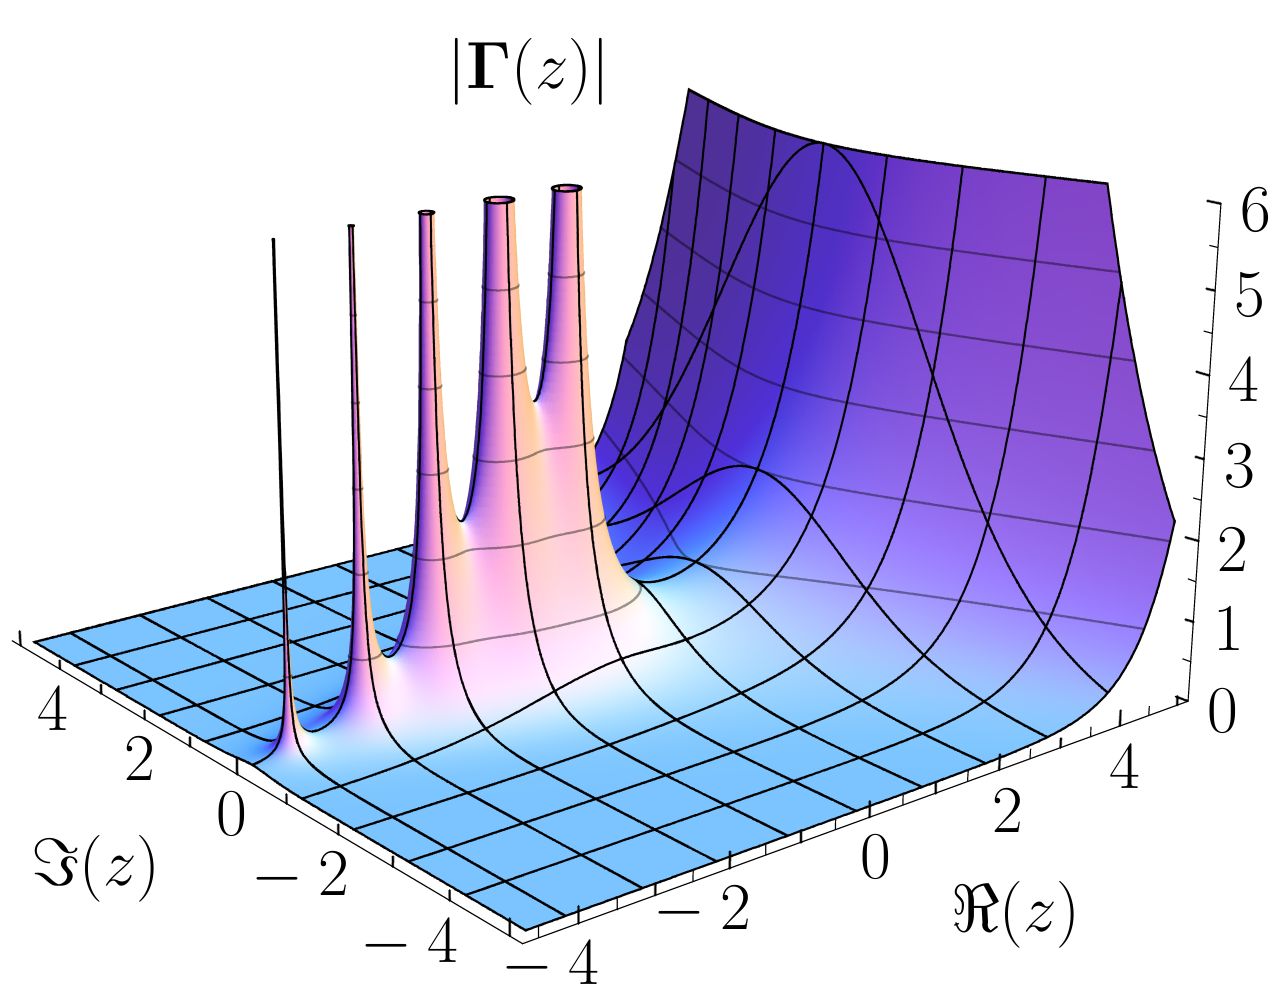
\includegraphics[scale=0.2]{abs_gamma}
		\caption{One can see the poles of $\Gamma(z)$ at $\Z_{<0}$. It is meromorphic.}
	\end{center}
\end{figure}

Jahnke and Emde's book\footnote{See \underline{Tables of Functions with Formulae and Curves} fig. 5, fig. 49, fig. 55, fig. 150, etc.} illustrates functions such as the gamma function, Jacobi/Weierstrass elliptic functions, and the Riemann zeta function. (Order-two poles are ``fatter'' than order-one poles.)

A function with an essential singularity is $f(z)=\sum_{k\in \Z}a_kz^k$ in which the number of terms with a negative exponent might not be finite. Expanding $e^{1/z} +e^z$ as a Laurent series, you see that something like this occurs. Any function with an essential singularity has this property.\footnote{See \url{https://youtu.be/MbPOKnwgL-8?t=702}.}

\begin{figure}
	\begin{center}
		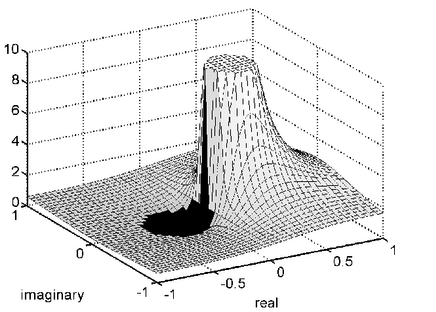
\includegraphics[scale=0.6]{exp_z_inv}
		\caption{An illustration of the essential singularity of $\exp(1/z)$.}
	\end{center}
\end{figure}

The function $\exp(1/z)$ has an essential singularity, and so does $\exp(-1/z^2)$.

If $f$ has an essential singularity at $0$, then $\{f(z):0<\abs{z}<\varepsilon\}$ is dense in $\C$. Suppose $\alpha$ is not a limit point of values of $f(z)$. Then $\abs{f(z)-\alpha} > \delta$, so $\abs{1/(f(z)-\alpha)}$ is bounded, and $1/(f(z)-\alpha)$ is holomorphic. (See Great Picard's theorem.)

Now we're on to non-isolated singularities. Limits of singularities are one: Take, for example,
 \begin{align*}
	f(z) = \frac{1}{\sin (1/z)}.
\end{align*}
Branch points are another: Take $\log z$ or $z^s$ (where $s\notin \Z$). Hankel functions are another example. Values change depending on from where you approach the point.

Then, we have natural boundaries. The function $f(z) = \sum_k z^k$ converges for $\abs{z} < 1$. It has a pole at $z=1$, but it is nonsingular elsewhere because we can continue it to a holomorphic function by $z/(1-z)$. Now consider $f(z) = \sum_k z^{2^k}$. There's obviously a pole at $z=1$. At $z=-1$, there's also a pole. At $z=i$? Pole. For all $2^k$th roots of unity, there is a pole. But $\abs{f(z)}$ does not tend to $\infty$ as $\abs z $ tends to $1$. If you approach a non--$2^k$th root of unity, we do not need to tend to $\infty$ at all. This is a natural boundary---a sort of ``wall of poles.''

\section{Gamma function}
Euler defined the gamma function as follows:
\begin{align*}
	\Gamma(s) := \int_0^\infty e^{-t} t^{ s-1} \, dt.
\end{align*}
It has the fundamental properties that
\begin{align*}
	s\Gamma(s) = \Gamma (s+1)
\end{align*}
and 
\begin{align*}
	\Gamma(1)=1.
\end{align*}
\iffalse Euler also wrote
\begin{align*}
	n! = \int_0^1 (-\log x)^n \, dx.
\end{align*}\fi
This defines a holomorphic function for $\Re s > 0$. Using its defining properties, one can extend it to a holomorphic function with poles at nonpositive integers.

Analyzing Figure 2, one notices that the poles of $\Gamma(s)$ get thinner as $s$ gets more negative. Further, $\abs{\Gamma(s)}$ seems to get smaller as $\abs{\Im s}$ increases. Wherefore?

The pole at $s=0$ has residue $1$, since $\Gamma(s) = s\inv \Gamma (s+1)$ and $\Gamma(1)=1$. At $s=-1$, since $\Gamma(s-1)= (s-1)\inv\Gamma (s)$ and the previously-mentioned pole has residue $1$, the pole has residue $1/(-1) = -1$. At $s=-2$, since $\Gamma(s-2)= (s-2)\inv \Gamma(s-1)$, the pole has residue $(-1)/ (-2) = 1/2$. At $s=-3$, the residue is $-1/6$. One sees that at $s=-n$, the pole has residue $(-1)^n/n!$.

Further,
\begin{align*}
	\abs{\Gamma(s)} &= \abs{ \int_0^\infty e^{-t}t^{s-1}\, dt}\\
			&\le \int_0^\infty \abs{e^{-t}t^{s-1}}\, dt\\
			&= \int_0^\infty e^{-t} t^{\Re(s-1)}\, dt\\
			&= \Gamma (\Re s).
\end{align*}
So $\Gamma(s)$ is bounded for $\alpha \le \Re s \le \beta$ where $0<\alpha<\beta$, since $\Gamma(s)$ is bounded for $\alpha \le s \le \beta$. Now $\Gamma(s)=s\inv\Gamma (s+1)$, and $\Gamma(s+1)$ is bounded for $\alpha \le \Re s\le \beta$, so $s\inv\Gamma(s+1)$ tends to $0$ as $\abs{\Im s}$ tends to infinity. And $\abs{(\Im s)^n \Gamma (s)}$ is bounded for $n>0$. So $\Gamma(s)$ is rapidly decreasing in vertical strips $\alpha\le\Re s\le \beta$.

\begin{proposition}[Euler's reflection formula]\label{}\text{}
\[
	\Gamma(s)\Gamma (1-s) = \frac{\pi}{\sin  (\pi s)}
\]
\end{proposition}
\begin{proof}
\text{}
\begin{enumerate}
	\item Write $\varphi(s) := \Gamma (s)\Gamma (1-s)$. Notice that $\varphi(s) = - \varphi (s+1)$. Also, $\varphi$ has a pole of residue $1$ at $s=0$. Further, $\varphi(s)$ is rapidly decreasing in vertical strips $\alpha\le\Re s\le \beta$ where $\Im s>\varepsilon$. The same is true for $\pi/\sin(\pi s)$. Therefore, $\psi(s) :=  \varphi(s) - \pi/\sin (\pi s)$ satisfies $\psi(s+1)=-\psi (s)$, is rapidly decreasing, and has no poles: it is holomorphic everywhere. Since $\psi$ is periodic and bounded in vertical strips, it is bounded. Therefore, by \cref{lvl} (Liouville), $\psi$ is constant. Since both functions are rapidly decreasing, $\psi = 0$.
	\item \begin{align*}
			\Gamma(s)\Gamma (1-s) &=  \int_0^\infty e^{-t}t^{s-1} \, dt \int_0^\infty e^{-u} u^{1-(s-1)}\, du\\
					      &= \int_0^\infty\int_0^\infty e^{- (t+u) } (t/u)^s t\inv \, dt\, du\\
					      &= \int_0^\infty \int_0^\infty e^{-u (t+1)} t^s t\inv \,dt\,du&t\longmapsto tu\\
					      &= \int_0^\infty \frac{1}{t+1} t^{s-1} \,dt\\
					      &= \frac{\pi}{\sin  (\pi s)} & \textrm{\cref{ibc_1}.} 
	\end{align*}
\end{enumerate}
\end{proof}

\begin{remark}
	A theme of Riemann: To study a complex function, you should analyze its singularities and growth rate.
\end{remark}

\begin{remark}
		$\Gamma(1/2) = \sqrt{\pi}$.
\end{remark}
\begin{remark}
		$\Gamma(s)\ne 0$.
\end{remark}
\begin{proposition}[ ]\label{}\text{}
The function $\Gamma(s)$ is the only meromorphic function such that
\begin{enumerate}
	\item $s\Gamma(s) = \Gamma (s+1)$;
	\item $\Gamma(s)$ is bounded in strips $\alpha\le \Re s \le \beta$ where $\Im s \ge 1$;
	\item $\Gamma(1)=1$.
\end{enumerate}
\end{proposition}
\begin{proof}
Suppose $\Gamma_0$ has these properties. Then 
\begin{align*}
	\Gamma_0(s)\Gamma (1-s) = \frac{\pi}{\sin  (\pi s)}
\end{align*}
since the proof of the reflection formula only required the three properties in question. Hence $\Gamma_0 = \Gamma$. 
\end{proof}

The function $\varphi(s) :=\Gamma(s/2)\Gamma ((s+1) /2)$ has the ``same poles'' as $\Gamma(s)$. Now
\begin{align*}
	\varphi(s+1)& = \Gamma((s+1)/2) \Gamma(s/2 + 1)\\
		    &= (s/2)\Gamma ((s+1)/2) \Gamma(s/2)\\
		    &=  (s/2)\varphi (s).
\end{align*}
Now, set $\psi(s):=2^s\Gamma(s/2)\Gamma ((s+1) /2) $. Then $\psi(s+1)=s\psi (s)$. The function $\psi$ is bounded in vertical strips (except near poles, as with $\Gamma$). So $\psi(s) = \alpha\Gamma (s)$ for some constant $\alpha$. Now, with $s=1$, we find
\begin{align*}
	2^1 \Gamma(1/2)\Gamma (1) &= \alpha \Gamma (1)\\
	\alpha &= 2\sqrt{\pi}.
\end{align*}
Therefore,
\begin{align*}
	2^s\Gamma(s/2)\Gamma((s+1) /2) = 2\sqrt \pi \Gamma(s).
\end{align*}
(This is called the duplication formula.)

 \begin{exercise}\label{extend it}\text{}
Prove that
\begin{align*}
	m^s \prod_{k=1}^m \Gamma \left(\frac{s+ k - 1}{m} \right) = (2\pi)^{ (m-1)/2} \sqrt m \Gamma (s).
\end{align*}
\end{exercise}

\section{Maximum modulus principle}

Suppose $f$ is holomorphic and $U$ is an open set. If $\abs{f(z)}$ is maximal at $z\in U$ then, $f$ is constant.

\begin{proof}
Suppose $f(z)$ is maximal at $z=0$. Let $C$ be a curve around $0$. Then
 \begin{align*}
	 f(0)& = \frac{1}{2\pi i} \int_C \frac{f (z)}{z}\, dz\\ 
	     &= \frac{1}{2\pi i} \int_0^{2\pi} \frac{f(re^{i\theta})}{re^{i\theta}} ire^{i\theta}\, d\theta\\
	     &= \frac{1}{2\pi} \int_0^{2\pi} f (re^{i\theta}) \, d\theta\\
	     &= \textrm{average of $f$ on $C$.}
\end{align*}
Suppose $\abs{f(0)} = M$, so $\abs{f(z)}\le M$. But $f(0)$ is the average of $f$ on $C$, so $f(z)=f (0)$ for all $z$ on $C$. So $f$ is constant. 
\end{proof}

There is a physical interpretation. Recall that if $f$ is holomorphic, then $\Re f$ is harmonic, so it satisfies the steady-state heat equation. Think of a plate $U$. The heat at a point of maximum temperature on $U$ will flow out to cooler areas. So the heat must be the same throughout the plate.

\begin{theorem}[Fundamental theorem of algebra]\label{}\index{}\text{}
Any non-constant polynomial $f$ has a root.
\end{theorem}
\begin{proof}
Suppose $f$ has no root and $f(0)=M$. Then $1/f(z)\to 0$ as $\abs{z} \to\infty$ and $1/f(z)$ is holomorphic. Then pick the maximum value of $f(z)$ for $\abs{z}\le M/2$, which you can do since we're dealing with a continuous function on a compact region. Further, $f$ cannot be constant since it tends to $0$, so we obtain a contradiction: $1/f(z)$ is not holomorphic, so $f$ vanishes somewhere.

One might also use Liouville's theorem.
\end{proof}

Consider $U=\{z\in \C :\abs z < 1\}$. One symmetry of $U$ is given by $z\longmapsto \exp(i\theta)z$, which rotates $U$ by $\theta$. Any symmetry is a map $f:U\longrightarrow U$ that is holomorphic with an inverse $f\inv : U\longrightarrow U$. One can check that
\begin{align*}
	f(z) = \frac{z-\alpha}{1-\ol\alpha z}
\end{align*}
is another symmetry for $\abs\alpha < 1$. We get a three-dimensional group of symmetries given by 
\begin{align*}
	z \longmapsto \exp(i\theta) \frac{z-\alpha}{1-\ol\alpha z}.
\end{align*}
(These are called M\"obius transformations.) Are there others?

Suppose $f:U\longrightarrow U$. We can compose $f$ with a M\"obius transformation to make $f(0)=0$. Now put $g(z):=f (z)/z$. The function $g$ is holomorphic since it has a removable singularity at $0$. We want to show that if $\abs{z}<1$, then $\abs{g(z)}\le 1$ (where $=$ occurs only if $g$ is constant). Now $\abs{g(0)} \le 1$, and if $\abs{g(0)} = 1$, then $g$ is constant by the maximum modulus principle. Suppose that $f$ has an inverse $f\inv : U\longrightarrow U$ with $f(0)=0$. Then 
\begin{align*}
	f'(0) = \frac{1}{ (f\inv)'  (0)},
\end{align*}
and $f'(0)$ and $(f\inv)' (0)$ have absolute value at most $1$, so $\abs{f'(0)} = 1$. And $f'(0)=g (0)$, so $g$ is constant and $f$ is linear. Therefore, $f(z)=\exp (i\theta)z$. That is, all symmetries of $U$ are M\"obius transformations.

What about the structure of this group? First, notice that we can identify it with the upper half-plane by
\begin{align*}
	w &\longmapsto \frac{z-i}{z+i}\\
	i\frac{1+w}{1-w} &\longmapsfrom z.
\end{align*}
So we get a group of three-dimensional symmetries of the upper half-plane. These are given by $\PSL_2(\R)$, which acts on the upper half-plane by 
\begin{align*}
	\mat{a&b\\c&d}(\tau) = \frac{a\tau + b}{c\tau +d}.
\end{align*}
The more profound idea here is to find a group $\Gamma\subseteq \PSL_2(\Z)$ and look for functions on $\H$ invariant under $\Gamma$ (these are called modular functions). 

\section{Elliptic functions}
Elliptic functions are doubly-periodic functions. Recall that a doubly-periodic function $\varphi$ satisfies $\varphi(z) = \varphi (z+\omega_1) = \varphi  (z+\omega_2)$ for two $\R$--linearly independent numbers $\omega_1,\omega_2\in \C$. 

Are there holomorphic elliptic functions? Well, no: If $\varphi$ is holomorphic and elliptic, then it is constant, since $\varphi$ is bounded in the fundamental domain in the lattice generated by two linearly independent periods (which is compact if you include the boundary points) and $\varphi$ is continuous. That is, $\varphi$ is bounded on $\C$ by periodicity. So, by \cref{lvl}, $\varphi$ is constant.

Let's find a meromorphic function $\varphi$ such that $\varphi(z) = \varphi (m\omega_1 + n\omega_2 + z)$ for all $m,n\in\Z$ (that is, $\varphi$ is doubly-periodic). Here, we get a group of translations isomorphic to $\Z\oplus\Z$. A straightforward way to get a function $\varphi$ invariant under a group is to take the average of some function $\psi$:  
 \begin{align*}
	\varphi(z) = \sum_{m,n\in \Z} \psi (z+m\omega_1 + n\omega_2).
\end{align*}
So, we have an elliptic function---right? Wrong! This function $\varphi$ is elliptic if the series is absolutely convergent. Let's figure out when that is the case.

Suppose that $\psi(z)\le \textrm{constant}/z^\alpha$ for $\abs z$ large. We will estimate the sum in an annulus. Fix a natural number $r$. Then the number of points in the annulus $\{z : \abs{z} < r+1\} - \{z : \abs{z} < r\}$ of the form $m\omega_1 + n\omega_2$ is at most a constant times $r$. So the sum is bounded by $\sum _{r\in \N} \textrm{constant}\, r/r^\alpha$, which converges for $\alpha>2$.

Now if $\psi$ is a rational function of degree at most $-3$, then it is elliptic. For instance,
\begin{align*}
	\psi(z) := \frac{1}{ (z-\alpha) (z-\beta) (z-\gamma)}
\end{align*}
has poles at $\{\alpha,\beta,\gamma\}+m\omega_1 + n\omega_2$. That is, we need at least $3$ poles in the fundamental domain. 

But are there elliptic functions with $1$ or $2$ poles in the fundamental domain? Notice that an elliptic function $\varphi$ is determined by its roots and poles up to constant multiplication. 

One requires the argument principle. Suppose $f$ is meromorphic in a region $U$. Write $f(z) = a_nz^n+\cdots$, so $f'(z) = na_nz^{n-1} + \cdots$. Then $f'(z)/f (z) = nz\inv + \cdots$, and the first term has residue $n$, which is the order of the root of $f$ at $0$. Then 
\begin{align*}
\frac{1}{2\pi i} \int_{\partial U} \frac{f'(z)}{f (z)} \, dz &= \# \textrm{roots} - \#\textrm{poles} \\
							     &= \frac{1}{2\pi}\Delta (\arg f(z)).
\end{align*}
Why? Well, 
\begin{align*}
	\frac{f'(z)}{f (z)} = \frac{d}{dz} (\log  f(z)),
\end{align*}
and even though $\log$ is multivalued, it changes by a constant, but differentiating kills that constant. So that integral above is $(1/2\pi i)\times \Delta  (\log f(z))$. But $\log$ only changes in its imaginary part around this contour, so we get the result above.

Now, suppose $f$ is elliptic. How many roots and poles does it have in its fundamental domain? Well,
\begin{align*}
	(\#\textrm{roots} - \#\textrm{poles})\Big |_{\textrm{fundamental domain}}& = \frac{1}{2\pi i} \int_{\partial(\textrm{fundamental domain})} \frac{f' (z)}{f (z)}\, dz.
\end{align*}
But $f(z)=f (z+\omega_1) = f(z+\omega_2)$, and we are integrating along the fundamental domain, so the integrals on its parallel sections cancel. Hence
\begin{align*}
	\#\textrm{roots} = \#\textrm{poles}
\end{align*}
is in the fundamental domain. Now, if a root or pole is on the boundary of the fundamental domain, we slightly manipulate the contour of integration to avoid the root/pole. Therefore, we only count a root/pole once if it is on the boundary. Do not over-count! 

Let's take this further. With the residue calculus, we see that
\begin{align*}
	\frac{1}{2\pi i} \int_C \frac{f'(z)}{f (z)} g (z)\, dz = \sum_{\textrm{roots/poles $p$}} \Res (f'/f, \,p) g (p)
\end{align*}
if $g$ is holomorphic. Now, suppose $f$ is elliptic. Then
\begin{align*}
	\frac{1}{2\pi i} \int_C \frac{f'(z) }{f(z) } z\, dz &= \frac{1}{2\pi i} \left( \int_{\omega_1}^{\omega_1+\omega_2} \frac{f'(z) }{f(z) } z\, dz - \int_0^{\omega_2}\frac{f'(z) }{f(z) } z\, dz +\textrm{similar} \right)\\
							    &= \frac{1}{2\pi i} \left( \int_0^{\omega_1} \frac{f'(z) }{f(z) } ((z+\omega_1) - z) \, dz + \textrm{similar} \right)\\
							    &= \frac{1}{2\pi i} \left( \omega_1 \int_0^{\omega_2} \log f(z)\, dz + \omega_2 \int_0^{\omega_1} \log f(z) \, dz\right)\\
							    &= m\omega_1 + n\omega_2 &m,n\in \Z.
\end{align*}
Therefore, 
\begin{align*}
	\sum_{\textrm{roots/poles $p$}} p \Res(f'/f, p) = m\omega_1+n\omega_2
\end{align*}
for some integers $m$ and $n$.

Let's show that $f$ cannot have exactly $1$ pole. Suppose $f$ has a pole at $\alpha$ and a root at $\beta$. Then $\alpha-\beta = m\omega_1+n\omega_2$. This is saying that (supposing $f$ has a pole at $\alpha$) that $f$ has both a pole and a root at $\alpha$, which is a contradiction.

What about $2$ poles in the fundamental domain? Write $n_p := \Res(f'/f, p)$. Then we have the following conditions for an elliptic function:
\begin{itemize}
	\item $\sum n_p = 0$;
	\item $\sum p n_p = m\omega_1+n\omega_2$. 
\end{itemize}
These are sufficient conditions. In fact, we can have $2$ poles for an elliptic function. 
\section{Weierstrass elliptic functions}
If we want an elliptic function with a pole of order $3$ at $0$, we might take
\begin{align*}
	\sum_{m,n\in\Z}^{} \frac{1}{(z+m\omega_1+n\omega_2)^3}.
\end{align*}
This is okay, but, for a pole of order two, we cannot take
\begin{align*}
	\sum_{m,n\in\Z}^{} \frac{1}{(z+m\omega_1+n\omega_2)^2}
\end{align*}
because this does not converge absolutely. Forevermore, 
\begin{align*}
	\lambda := m\omega_1+n\omega_2 \in \Lambda
\end{align*}
for a lattice $\Lambda$. Now, near $z=0$,
\begin{align*}
	\frac{1}{(z+\lambda^2)}\approx \frac{1}{\lambda^2},
\end{align*}
so we can try to subtract this ``divergent part'':
\begin{align*}
	\sum_{\lambda\in\Lambda}^{} \left(\frac{1}{(z+\lambda) ^2} - \frac{1}{\lambda^2}\right).
\end{align*}
What about at $\lambda = 0$, though? Second patch:
\begin{align*}
	\frac{1}{z^2} + \sum_{\lambda\in\Lambda-\{0\}}^{} \left( \frac{1}{(z+\lambda) ^2}-\frac{1}{\lambda^2} \right) .
\end{align*}
The summand is, approximately, of degree $-3$ in $\lambda$, so it converges absolutely. Let $\Lambda$ be a lattice. Then, we define
\begin{align*}
	 \wp (z) :=  \frac{1}{z^2} + \sum_{\lambda\in \Lambda-\{0\}} \left( \frac{1}{(z+\lambda) ^2}-\frac{1}{\lambda^2} \right). 
\end{align*}
But, now, this is not invariant under $z\longmapsto z+\lambda$---right? Well, it actually is:
\begin{align*}
	\wp'(z) = -2\sum_{\lambda\in\Lambda-\{0\}}^{} \frac{1}{(z+\lambda) ^2}.
\end{align*}
Term-by-term differentiation is valid: $\wp$ is locally uniformly convergent, local uniform convergence preserves integrals, and the derivative variation on the Cauchy integral formula shows that a derivative can be written as an integral. Therefore, 
\begin{align*}
	\wp(z) - \wp (z+\omega_1) = \alpha.
\end{align*}
The function $\wp$ is even, so, letting $z=-\omega_1/2$, $\alpha = 0$. Therefore,
\begin{align*}
	\wp(z) = \wp (z+\omega_1) = \wp(z+\omega_2).
\end{align*}
That is, $\wp$ is elliptic, and it has a pole of order $2$ at $z=0$. 

Abiding by this procedure for a pole of order $1$, we get
\begin{align*}
	\zeta(z) :=  \frac{1}{z} + \sum_{\lambda\in \Lambda-\{0\}}^{} \left( \frac{1}{z-\lambda}+ \frac{1}{\lambda} + \frac{z}{\lambda^2} \right), 
\end{align*}
which is Weierstrass's $\zeta$ function---not Riemann's. It is absolutely convergent and has a pole of order $1$. Now, let's continue to check if it's elliptic:
\begin{align*}
	\zeta'(z) = -\wp (z),
\end{align*}
so 
\begin{align*}
	\zeta(z+\omega_1) - \zeta(z) = \beta.
\end{align*}
Now, $\zeta$ is odd, and $\beta\ne 0$. So $\zeta$ is ``elliptic up to constants.''

Nevertheless, 
\begin{align*}
	\zeta(z-\alpha) - \zeta (z-\beta)
\end{align*} 
is elliptic. 

The function $\zeta$ defined this way is an example of a Mittag--Leffler series.

Any elliptic function with no poles is constant, and this fact generates legions of identities.\footnote{See \underline{A Course of Modern Analysis}.} Some light hand-waving\footnote{See \url{https://youtu.be/p1dts9PrDtI?t=1243}.} shows that
\begin{align*}
	(\wp'(z)) ^2 = 4(\wp(z)) ^3 - g_2\wp(z) -  g_3.
\end{align*}

\section{Classification of elliptic functions}
We can classify elliptic functions in three ways:
\begin{enumerate}
	\item They are all rational functions of $\wp$ and $\wp'$;
	\item They are determined by their roots and poles (up to a constant); 
	\item They are determined by their singularities (up to a constant).
\end{enumerate}

Suppose $f$ is elliptic. Notice that $f$ is the sum of an odd function and an even function. But an odd function divided by $\wp'$ is even, so this all reduces to the case when $f$ is even. 

Then, we get rid of all poles not on $\Lambda$ by multiplying by $\wp(z) -\wp (\alpha)$ (if there is a pole at $z=\alpha$).

Now, for the pole at $0$, we note that $f(z) = a_n z^{-2n} + \cdots$, and then we can write 
\begin{align*}
	f(z) = a_n \wp(z)^n + \textrm{something with a smaller pole}.
\end{align*}
We can continue to reduce the size of the pole by subtracting polynomials in $\wp$ until $f$ is zero. So every elliptic function is a rational function of $\wp$ and $\wp'$.

Recall that
\begin{align*}
	(\wp'(z)) ^2 = 4(\wp(z)) ^3 - g_2\wp(z) -  g_3.
\end{align*}
If $y=\wp'(z)$ and $x = \wp(z)$, we get a map 
\begin{align*}
	\C/\Lambda &\longrightarrow C:y^2 = 4x^3 -g_2x-g_3\\
	  z &\longmapsto (\wp(z),\wp' (z)).
\end{align*}
This is almost an isomorphism, except $0$ is taken to the point at infinity. 

The second classification: An elliptic function $f$ is determined by its roots and poles. Suppose $f$ has roots at $z=p_i$ of order $n_i$ (if $n_i<0$ then $f$ has a pole of order $-n_i$ at $z=p_i$). Some time ago, we put some conditions on these roots and poles:
\begin{enumerate}
	\item \begin{align*}
		\# \textrm{roots} = \# \textrm{poles} \iff \sum_{i}^{} n_i=0;
	\end{align*}
\item \begin{align*}
	\sum_{i}^{} p_in_i \in \Lambda.
\end{align*}
\end{enumerate}
We showed that these are necessary for $f$ to exist, but, now, it's time to show that they are sufficient. 

Recall that Weierstrass's zeta function has poles of order $1$ at $\lambda\in \Lambda$ and $\zeta' (z) = -\wp (z)$. Weierstrass's sigma function is defined by
\begin{align*}
	\sigma(z) := \exp  \left( \int_{\alpha}^{z} \zeta(z)  \, dz  \right) 
\end{align*}
or\footnote{See \url{https://mathworld.wolfram.com/WeierstrassSigmaFunction.html}.}
\begin{align*}
	\frac{d}{dz}\log \sigma(z):=  \zeta (z) 
\end{align*}
and
\begin{align*}
	\lim_{z\to 0} \frac{\sigma(z)}{z} := 1.
\end{align*}
The integral has logarithmic singularities at $\Lambda$, but these ``ambiguities'' are nullified by taking $\exp$. This function has roots of order $1$ at $\Lambda$ and no other roots or poles. It is not elliptic, but it satisfies
\begin{align*}
	\sigma(z + 2\omega_1) &= -\sigma(z)\exp(2\eta_1(z+\omega_1)) ;\\
	\sigma(z+2\omega_2) &= -\sigma(z)\exp (2\eta_2(z+\omega_2)) ;
\end{align*}
where
\begin{align*}
	\eta_1 &:= -\frac{\pi^2\vartheta_1^{(3)}}{12\omega_1\vartheta_1'};\\
	\eta_2 &:= - \frac{\pi^2\omega_2\vartheta_1^{(3)}}{12\omega_1^2\vartheta_1'}- \frac{\pi i }{2\omega_1}.
\end{align*}
Dr. Borcherds writes this as
\begin{align*}
	\sigma(z+\omega_1) = \sigma(z) \exp (A_1z+B_1).
\end{align*}
Now,
\begin{align*}
	\prod_i \sigma(z-p_i) ^{n_i}
\end{align*}
has roots of order $n_i$ at $p_i$. Applying $z\longmapsto z+\omega_1$ gives \begin{align*}
	\prod_i \sigma(z-p_i) ^{n_i} \exp(A_1(z-p_i) + B_1) ^{n_i}.
\end{align*}
Since $\sum_{}^{} n_ip_i\in \Lambda$, write $\sum_{}^{} n_ip_i = 0$. This, along with $\sum_{}^{} n_i=0$, means that
\begin{align*}
	\prod_i \sigma(z-p_i) ^{n_i}
\end{align*}
is invariant under $z\longmapsto z+\omega_1$, so is elliptic (provided $\sum_{}^{} n_ip_i=0$). So we can find elliptic functions with given roots and poles if and only if they satisfy the two conditions in question.

\begin{exercise}\label{}\text{}
Show that
\begin{align*}
	\wp(z) - \wp (\alpha) = -  \frac{\sigma(z+\alpha)\sigma (z-\alpha)}{\sigma^2 (z)\sigma^2 (\alpha)}.
\end{align*}
(Hint: Do not use the definitions. Consider the roots and poles of both sides, show they are the same, and show that the constant by which they differ is $0$.)
\end{exercise}

Can we find an elliptic function with singularities at specified points in the fundamental domain? Not always: With an appropriate choice of contour $C$, we can make
\begin{align*}
	\frac{1}{2\pi i} \int_{C}^{} f(z)  \, dz = 0, 
\end{align*}
so 
\begin{align*}
	\sum_{\textrm{points $p$}}^{} \Res(f, p) = 0.
\end{align*}
This condition is sufficient. (Notice that this also proves that you cannot have an elliptic function with only $1$ pole of order $1$ in its fundamental domain.)

Notice that $\wp^{(n)} (z-\beta)$ has a pole of order $n+2$, so we can use these to kill poles of order greater than $1$. Now, recall that
\begin{align*}
	\zeta(z-\alpha) - \zeta (z-\beta)
\end{align*}
has poles of order $1$ at $\alpha$ and $\beta$. We use a function of this kind to ``move all poles to one point.'' Therefore, we can assume that the function has one pole of order $1$. Now, recall that the sum of the residues must be $0$, so $f$ must be holomorphic and constant.

These Weierstrass functions have trigonometric analogues in $1$-dimensional lattices.\footnote{See \url{https://en.wikipedia.org/wiki/Weierstrass_functions}.} Recall:
\begin{align*}
	\wp(z) =  \frac{1}{z^2} + \sum_{\lambda\ne 0}^{} \left( \frac{1}{(z-\lambda) ^2} - \frac{1}{\lambda^2} \right). 
\end{align*}
Similarly,
\begin{align*}
	\sum_{n\in\Z}^{} \frac{1}{(z-n\pi)^2} = \frac{1}{\sin^2z},
\end{align*}
and this can be seen by analyzing poles, periodicity, and behaviour as $\left\lvert \Im z \right\rvert$ grows. 

Integrating $\wp$, we get $-\zeta$, and integrating $-\csc^2z$, we get
\begin{align*}
	\frac{1}{z}+\sum_{n\ne 0}^{} \left( \frac{1}{z-n\pi}+ \frac{1}{n\pi} \right) = \frac{1}{\tan z}.
\end{align*}

Finally, integrating and exponentiating $\zeta$, we get $\sigma$. Doing the same to $\cot z$, we get
\begin{align*}
	z\prod_{n\ne 0} \left( 1-\frac{z^2}{n^2\pi^2} \right) = \sin z.
\end{align*}
(Recall that Euler used this informally to resolve the Basel problem.)
\printindex
\end{document}
